% Câu 0, template cho một số công thức toán học và định đạng
\begin{tcolorbox}[
    colback=cyan!10!white,
    opacityback=0,
    enhanced jigsaw,
    colframe=black!75!white, 
    sharp corners]
    \textbf{Bài 0. (0 điểm)} % Nhập đề bài từ dòng kế tiếp
    Đây là câu hỏi mẫu, chứa template cho một số công thức toán học và định dạng. Khi biên tập vui lòng tuân theo các định dạng và chỉ dẫn.
\end{tcolorbox}

\textcolor{black}{\textbf{Lời giải. }}
\begin{itemize}
  % \begin{multicols}{2}
      \item[\textcolor{black}{\textbf{a.}}] {
        % Nội dung tiểu mục bắt đầu ở dòng kế tiếp
        Công thức toán trong dòng văn bản thì để trong dấu \$, ví dụ $a^2 + b^2 = c^2$. Công thức toán trên một dòng riêng thì để trong dấu \$\$ và xuống dòng, ví dụ
        $$\det(A + B) \cdot \det(A) = \det\left((A + B)^T\right) \cdot \det(A).$$

        Nếu trên nhiều dòng và muốn đánh số, trong trường hợp chứa các biểu thức vói quan hệ bằng nhau, lớn hơn, nhỏ hơn liên tiếp thì dùng
        \begin{flalign*}
            &&\det(A + B) \cdot \det(A)  
            &= \det\left((A + B)^T\right) \cdot \det(A) 
            & ~ \\
            && ~ 
            &= \det(A^T + B^T) \cdot \det(A) 
            & \hfill (1) \\
            && ~ 
            &= \det(A^TA+ B^TA) 
            & ~ \\
            && ~ 
            &= \det(I + B^TA)
            & \hfill (2) \\
        \end{flalign*}
        hoặc trong trường hợp tương đương ($\iff$), hệ quả ($\implies$) của nhiều hệ thức thì dùng  
        \begin{flalign*}
            && ~  
            & (a + b)^2 = 0 
            & ~ \\
            && ~ 
            \iff & a^2 + 2ab + b^2 = 0
            & ~ \\
            && ~ 
            \iff & a^2 + b^2 = -2ab.
            & \hfill (3) \\
        \end{flalign*}

        Hết một công thức toán hoặc chuỗi công thức toán thì phải có chấm hoặc phẩy tùy ngữ cảnh.

        % Phải để trống một dòng trước dấu } khi kết thúc
      }

      \item[\textcolor{black}{\textbf{b.}}] {
        % Nội dung tiểu mục bắt đầu ở dòng kế tiếp
        Giữa các biến hoặc số có ngăn cách dấu phẩy thì phải dùng thêm $\,$ để tạo khoảng trắng, ví dụ $(a,\,b,\,c)$ .

        Dấu nhân không dùng $a . b$ mà phải dùng $a \cdot b$; dấu ba chấm trong phép nhân nhiều biểu thức thì dùng $a_1 \cdot a_2 \cdots a_n$; dấu ba chấm thể hiện còn nhiều ý thì dùng $a_1,\,a_2,\,\ldots,\,a_n$.

        Phân thức nên là $\dfrac{a}{b}$; trong trường hợp phân thức chứa phân thức thì phân thức nằm trong (nhỏ hơn) sẽ dùng $\frac{i}{j}$, ví dụ $x = \dfrac{x}{x + \frac{1}{x}}$.

        % Phải để trống một dòng trước dấu } khi kết thúc
      }

      \item[\textcolor{black}{\textbf{c.}}] {
        % Nội dung tiểu mục bắt đầu ở dòng kế tiếp
        Các ký hiệu về tập hợp các số như số thực $\mathbb{R}$, số phức $\mathbb{C}$; định thức ma trận $\det(A)$; chiều của không gian vector $\dim V$. 

        Các ký hiệu toán như hạng của ma trận, hạt nhân và ảnh của ánh xạ tuyến tính thì dùng $\text{rank}(A)$, $\text{Ker}f$ và $\text{Im}f$ do không có ký hiệu \LaTeX.

        % Phải để trống một dòng trước dấu } khi kết thúc
      }

      \item[\textcolor{black}{\textbf{d.}}] {
        % Nội dung tiểu mục bắt đầu ở dòng kế tiếp
        Hệ các hệ thức thì dùng 
        $$\left\{ \begin{matrix}[]{l}
            x + y = 0 \\ 
            x - y = 1
        \end{matrix} \right..$$

        Ma trận và định thức của ma trận thì dùng 
        $$\begin{pmatrix}[]{cc|c}
            a & b & c \\ 
            d & e & f
        \end{pmatrix} \text{ và } \begin{vmatrix}[]{cc}
          a & b \\ 
          d & e
        \end{vmatrix}$$
        chú ý rằng bao nhiêu cột thì khai báo bấy nhiêu cột ($c$ là center còn $l$ là left, $r$ là right).

        % Phải để trống một dòng trước dấu } khi kết thúc
      }

      \item[\textcolor{black}{\textbf{e.}}] {
        % Nội dung tiểu mục bắt đầu ở dòng kế tiếp
        Ký hiệu về tổng dãy số 
        $$\displaystyle \sum \limits_{i = 0}^n a_i = a_0 + a_1 + a_2 + \cdots + a_n$$ 
        và tích dãy số
        $$\displaystyle \prod \limits_{i = 0}^n a_i = a_0 \cdot a_1 \cdot a_2 \cdots a_n.$$ 

        Ký hiệu về giới hạn $\lim \limits_{n \to +\infty} a_n$.

        Ký hiệu về nguyên hàm $\displaystyle \int f(x) \mathrm{d}x$ và tích phân $\displaystyle \int \displaylimits_{a}^{b} f(x) \mathrm{d}x$. Chú ý rằng vi phân phải là $\mathrm{d}x$ chứ không phải $dx$.

        % Phải để trống một dòng trước dấu } khi kết thúc
      }

      \item[\textcolor{black}{\textbf{f.}}] {
        % Nội dung tiểu mục bắt đầu ở dòng kế tiếp
        Chèn file code vào file tài liệu:
        
        \lstinputlisting[language=C++, caption=]{./Resources/Files/code_sample.cpp}

        % Phải để trống một dòng trước dấu } khi kết thúc
      }
      
      \item[\textcolor{black}{\textbf{g.}}] {
        % Nội dung tiểu mục bắt đầu ở dòng kế tiếp
        Chèn bảng vào file tài liệu:
        
        \begin{table}[h]
            \centering
            \begin{tabular}{|C{3cm}|C{3cm}|C{3cm}|}
                \hline
                \bf ABC & \bf XYZ & \bf UVW \\

                \hline
                123 & 123 & 123 \\
                \hline
               123 & 123 & 123 \\
                \hline
            \end{tabular}
            \caption{Chèn bảng mẫu vào tài liệu với caption.}
            \label{tab:table-sample}
        \end{table}

        % Phải để trống một dòng trước dấu } khi kết thúc
      }

      \item[\textcolor{black}{\textbf{h.}}] {
        %%%%% Nội dung tiểu mục bắt đầu ở dòng kế tiếp
        Chèn hình ảnh vào file tài liệu:
        \begin{center}
            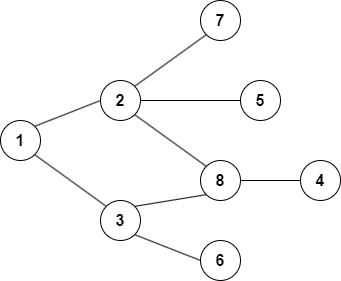
\includegraphics[scale=0.585]{./Resources/Images/image_sample.png}
        \end{center}

        Nếu muốn chèn caption, hãy dùng:
        \begin{figure}[ht]
            \centering
            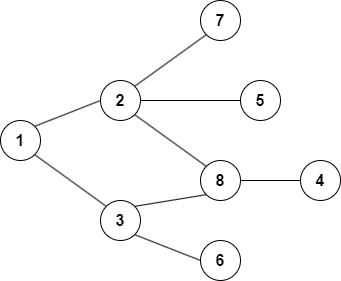
\includegraphics[scale=0.585]{./Resources/Images/image_sample.png}
            \caption{Chèn hình ảnh mẫu vào tài liệu với caption.}
            \label{fig:image-sample}
        \end{figure}
        
        %%%%% Phải để trống một dòng trước dấu } khi kết thúc
      }
  % \end{multicols}
\end{itemize}